% Figure 2: Technology Evolution Timeline
\begin{figure}[htbp]
\centering
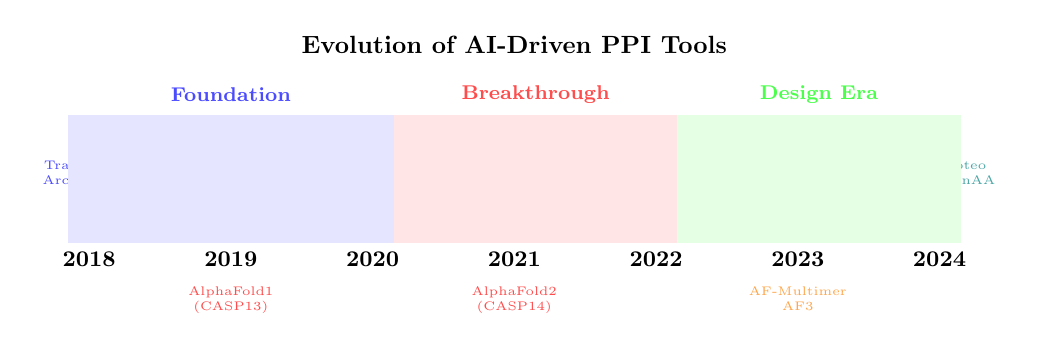
\begin{tikzpicture}[scale=0.9, transform shape]

% Timeline base
\draw[ultra thick, gray!70] (0,0) -- (12,0);

% Year markers
\foreach \x/\year in {0/2018, 2/2019, 4/2020, 6/2021, 8/2022, 10/2023, 12/2024} {
    \fill[gray!70] (\x,0) circle (4pt);
    \node[below, font=\small\bfseries] at (\x,-0.3) {\year};
}

% Milestones above timeline
\node[above, text width=1.5cm, align=center, font=\tiny] at (0,0.4) {
    \textcolor{blue!70}{Transformer}\\
    \textcolor{blue!70}{Architecture}
};

\node[above, text width=1.5cm, align=center, font=\tiny] at (4,0.4) {
    \textcolor{purple!70}{ESM-1b}\\
    \textcolor{purple!70}{(PLM)}
};

\node[above, text width=1.8cm, align=center, font=\tiny] at (8,0.4) {
    \textcolor{green!70}{ProteinMPNN}\\
    \textcolor{green!70}{RFdiffusion}
};

\node[above, text width=1.8cm, align=center, font=\tiny] at (12,0.4) {
    \textcolor{teal!70}{AlphaProteo}\\
    \textcolor{teal!70}{RFdiffusionAA}
};

% Milestones below timeline
\node[below, text width=1.5cm, align=center, font=\tiny] at (2,-0.8) {
    \textcolor{red!70}{AlphaFold1}\\
    \textcolor{red!70}{(CASP13)}
};

\node[below, text width=1.5cm, align=center, font=\tiny] at (6,-0.8) {
    \textcolor{red!70}{AlphaFold2}\\
    \textcolor{red!70}{(CASP14)}
};

\node[below, text width=1.8cm, align=center, font=\tiny] at (10,-0.8) {
    \textcolor{orange!70}{AF-Multimer}\\
    \textcolor{orange!70}{AF3}
};

% Phase regions
\fill[blue!10] (-0.3,-0.3) rectangle (4.3,1.5);
\fill[red!10] (4.3,-0.3) rectangle (8.3,1.5);
\fill[green!10] (8.3,-0.3) rectangle (12.3,1.5);

% Phase labels
\node[font=\footnotesize\bfseries, color=blue!70] at (2,1.8) {Foundation};
\node[font=\footnotesize\bfseries, color=red!70] at (6.3,1.8) {Breakthrough};
\node[font=\footnotesize\bfseries, color=green!70] at (10.3,1.8) {Design Era};

% Title
\node[font=\normalsize\bfseries] at (6,2.5) {Evolution of AI-Driven PPI Tools};

\end{tikzpicture}
\caption{Timeline of key technological advances in AI-driven protein-protein interaction research. The field has progressed through three phases: Foundation (2018-2020) with deep learning architectures, Breakthrough (2020-2022) with AlphaFold2, and Design Era (2022-present) with generative models for protein design.}
\label{fig:timeline}
\end{figure}
